\documentclass{article}

\usepackage{geometry, graphicx, subfiles, hyperref}
\newcommand{\margin}[2]{\geometry{  left = #1,
	right = #1,
	top = #2,
	bottom = #2} }
\margin{2cm}{3cm}

\usepackage{fancyvrb, lastpage, fancyhdr}
\usepackage{mathtools}
\pagestyle{fancy}
\rhead{RODD}
\lhead{Master Parisien de Recherche Opérationnelle}

\newcommand{\mailRef}[3]{\href{mailto:#3}{#1 \textsc{#2}}}

\newcommand{\pageDeGarde}[6]{
	\begin{titlepage}\center
		
		% --- Logo avant le titre --- %
		\begin{figure}
			\begin{center}
				#5
			\end{center}
		\end{figure}
		
		% --- sur titre -- %
		\textsc{\LARGE #2}\\ \vfill
		% --- titre --- %
		\rule[5mm]{\textwidth}{0.5mm} \\ \vfill
		{ \huge \bfseries\centering #1}\\ \vfill
		\rule[5mm]{\textwidth}{0.5mm} \\ \vfill
		
		% --- auteur --- %
		\begin{minipage}{0.4\textwidth}
			\begin{flushleft} \large
				\emph{Auteur :}\\ #3
			\end{flushleft}
		\end{minipage}
		\begin{minipage}{0.4\textwidth}
			\begin{flushright} \large
				\emph{Superviseurs:} \\ #4
			\end{flushright}
		\end{minipage}\\ \vfill
		
		% --- logo de fin --- %
		\rule{0.8\textwidth}{0.5mm} \vfill
		#6  \vfill
		{\large \today}
	\end{titlepage}
	\newpage
}


\begin{document}
	
	\pageDeGarde{ Projet RODD
	}{ Le Cnam \\ Institut Polytechnique de Paris 
	}{
		\mailRef{Justine}{De Sousa}{justine.desousa6@gmail.com}\\
		\mailRef{Vincent}{Maron}{vincent.maron@telecom-paris.fr}
	}{ \mailRef{Safia}{Kedad-Sidhoum}{safia.kedad_sidhoum@cnam.fr}
	}{ 
\includegraphics[width=0.8\textwidth]{logos/logo_ipp.png}
	}{ 
\includegraphics[width=0.8\textwidth]{logos/logoCnam.png}
	}
	
	\section{Modélisation de la contrainte intervalle glissant (Rolling)}
	La contrainte d'intervalle glissant est grandement similaire à une contrainte cumulative: plutôt que de faire la somme de 1 à $t$, on va la faire de $t$ à $t+R-1$. Dans notre cas, on prendra $f^m_t$ et $e^m_t$ stationnaires, indépendants de $t$, et $p_t^m = 1$ et $h_t(s_t) = s_t$.
	
	
	\huge{$$\sum_{t'=t}^{t+R-1} \sum_{m=1}^{M} (e^m-E)x_{t'}^{m}  \leq 0, \forall t\in \{1,...,T-R+1\} $$}
	
	\normalsize
	
	Ce qui nous donne le modèle suivant:
	\Large
	$$
	\begin{dcases}
		Min \sum_{t=1}^T (s_t + \sum_{m=1}^M f^m y_t^m )\\
		x_t^m \geq 0, &\forall t \in \{1,...,T\},  \forall m \in \{1,...,M\}  \\
		y_t^m \in \{0,1\}, &\forall t \in \{1,...,T\},  \forall m \in \{1,...,M\}  \\
		s_t \geq 0, &\forall t \in \{1,...,T\}\\
		s_t = s_{t-1} - d_t + \sum_{m=1}^M x_t^m \text{ avec $s_0 = 0$}&\forall t \in \{1,...,T\} \\
		x_t^m \leq M y_t^m \text{ avec $M = \sum_{t'=t}^T d_{t'}$}&\forall t \in \{1,...,T\},  \forall m \in \{1,...,M\}\\
		\sum_{t'=t}^{t+R-1} \sum_{m=1}^{M} (e^m-E)x_{t'}^{m}  \leq 0, &\forall t\in \{1,...,T-R+1\}\\
	\end{dcases}$$
	\newpage
	\section{Exemple}
	Pour l'instance:
	\begin{itemize}
		\item $T = 12$, $M = 4$
		\item $E_t^{max} = 3$
		\item $d_t = [40, 23, 63, 24, 53, 25, 25, 55, 34, 21, 47, 65]$
		\item $f^m = [10, 30, 60, 90]$
		\item $e^m = [8, 6, 4, 2]$
	\end{itemize}
	On obtient cette solution:\\
	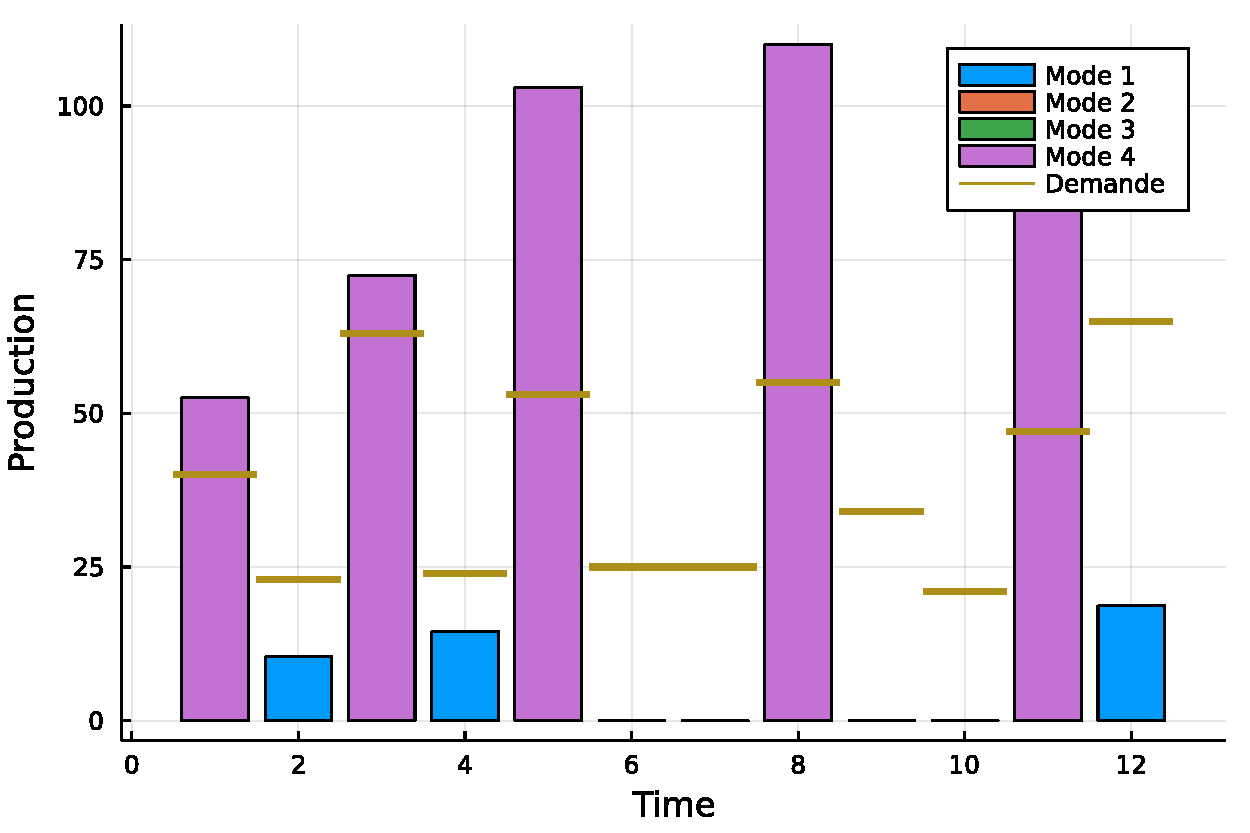
\includegraphics[width=\textwidth]{exemple.pdf}
	\normalsize
	On a un comportement attendu; comme $R$ ne vaut pas 1, on peut se permettre de ne pas produire uniquement dans des modes écologiques, ce qu'on peut observer à $t = 2,4,12$ où on produit en mode 1, sachant que $(f_1, e_1) = (10, 8)$. Pour tout autre $t$, on utilise le mode 4 avec $(f_4, e_4) = (90, 2)$. On note aussi que la solution fait régulièrement des stocks, puisque la production est souvent supérieure à la demande.\\
	\newpage
	\section{Influence des paramètres}
	Étant donné que plus R est bas, plus on se rapproche de la contrainte absolue où on ne peut produire qu'en écologique, et qu'à R=T on est le moins contraint dans le sens qu'on peut répartir les émissions carbone comme bon nous semble dans le temps, on peut se poser la question de l'influence de R sur le coût total et les émissions carbone moyennes.\\
	Pour l'instance précédente, on trace le coût total et la valeur de l'émission carbone moyenne en fonction de $R$.\\
	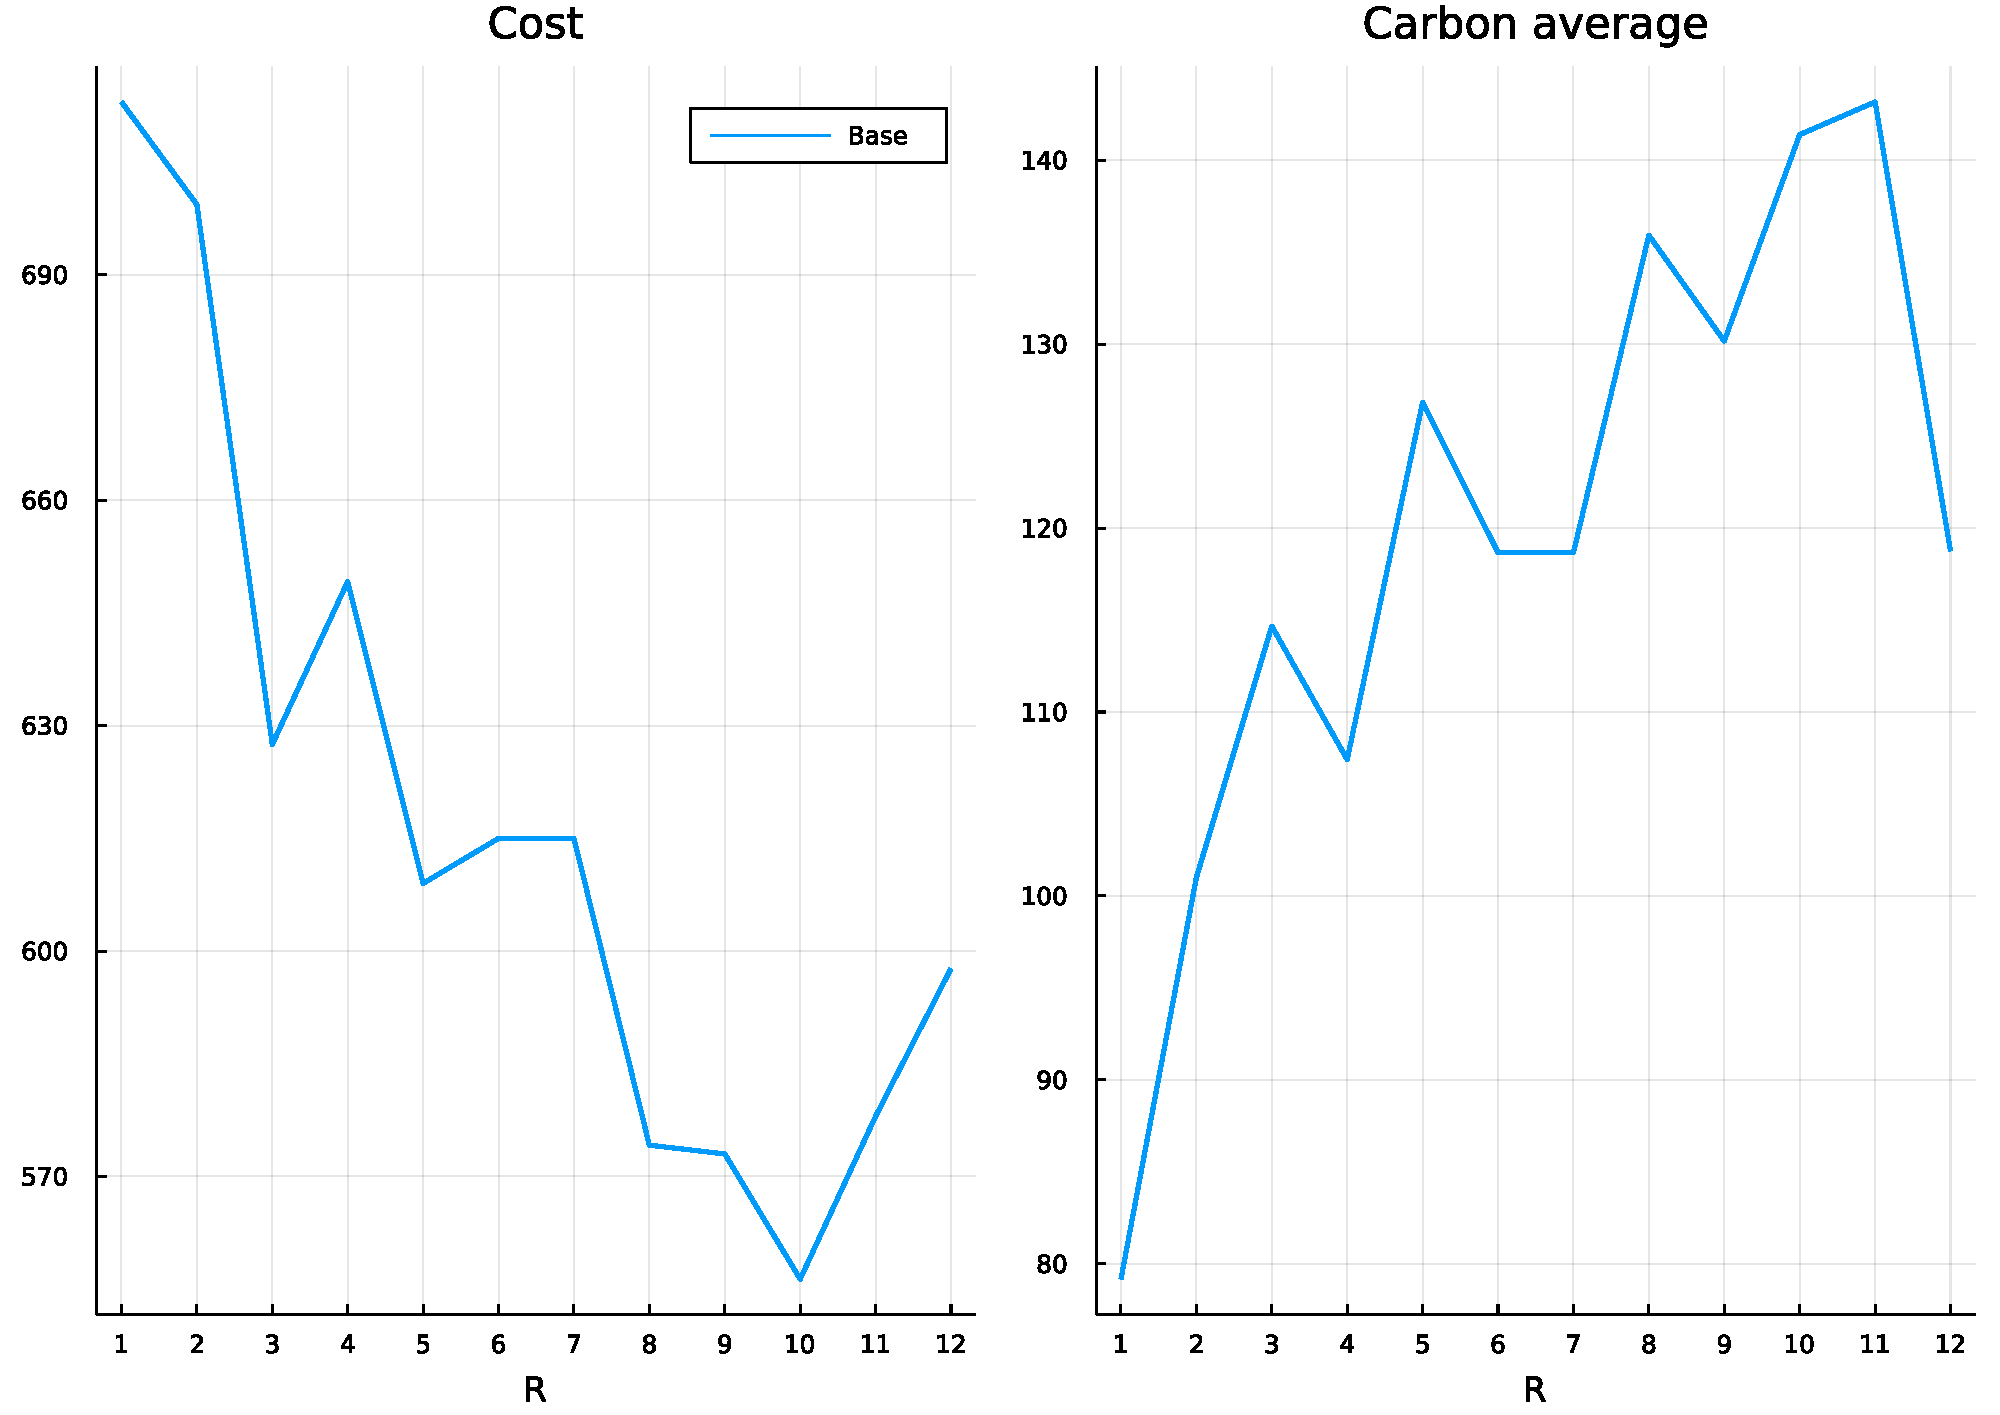
\includegraphics[width=\textwidth]{graph1.pdf}\\
	Que ce soit pour cette instance ou pour les autres testées, la tendance reste la même, il semblerait qu'à mesure qu'R augmente, la restriction sur le carbone est levée et donc, le coût de la solution baisse au détriment de l'émission carbone moyenne.\\
	\newpage
	Si on augmente E, on s'attendrait à ce que le coût des solutions baisse et que les émissions carbone augmentent fortement, et c'est effectivement ce qu'on observe:\\
	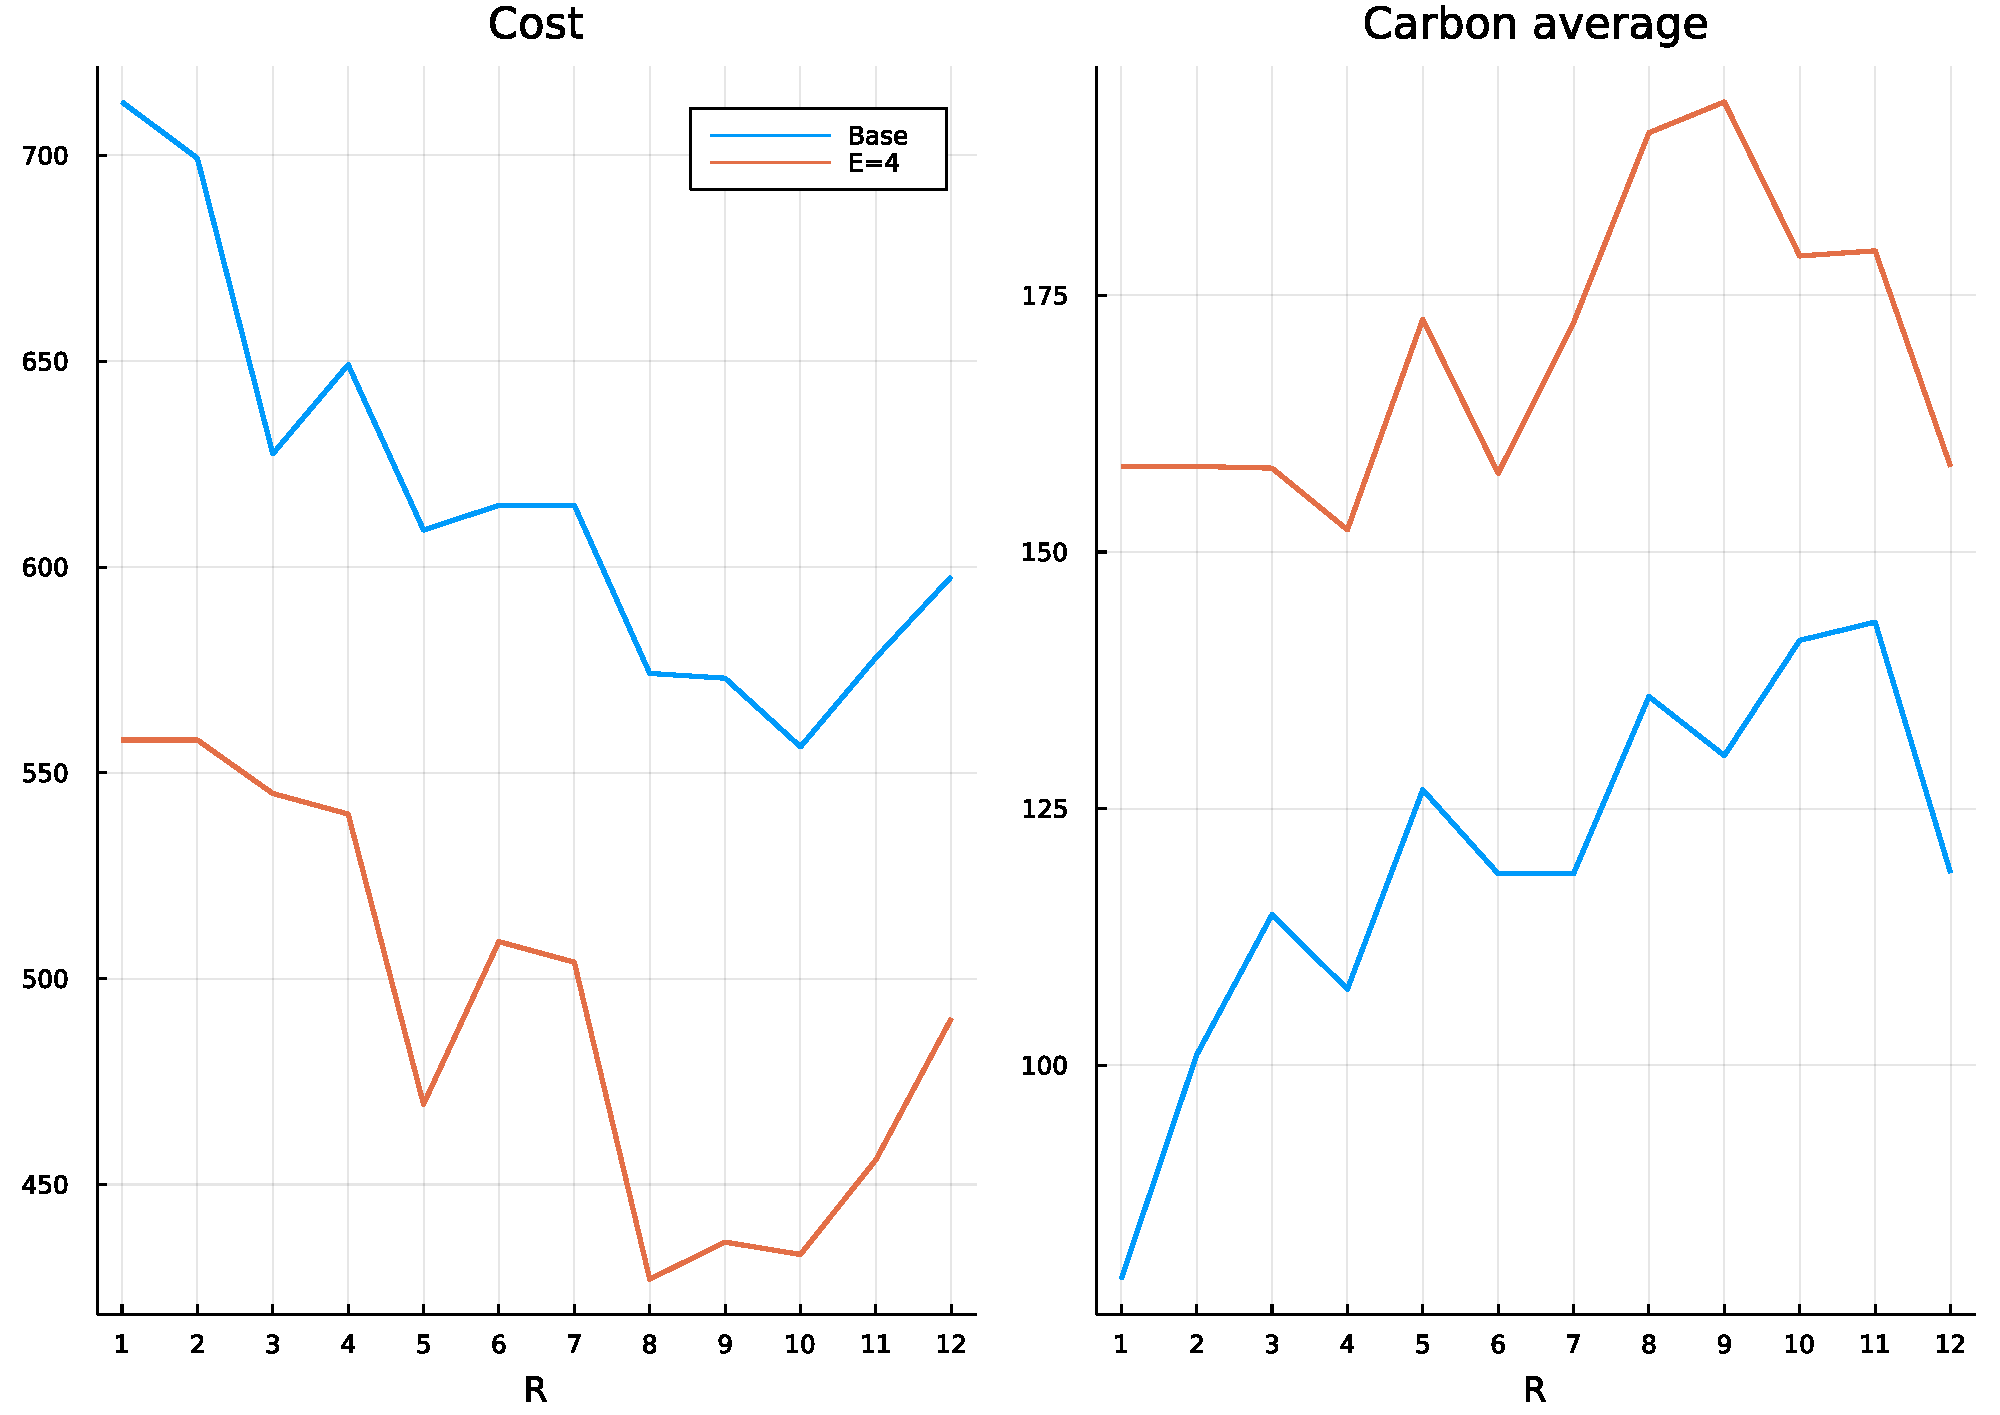
\includegraphics[width=\textwidth]{graph2.pdf}\\
	Maintenant, si on augmente le nombre de modes. On pourrait s'attendre à au moins 3 cas:\\
	\begin{itemize}
		\item Si le nouveau mode n'est pas utilisé. Ca serait a priori le cas par exemple d'un mode ni particulièrement écologique, ni particulièrement économique. Par exemple on peut imaginer qu'un mode de coût $f=50$ et d'émission $e=5$ ne changerait pas grand chose à l'instance actuelle.
		\item Si le nouveau mode est très écologique, il va être utilisé pour remplir les quotas et on peut s'attendre à des solutions de coût inférieur, mais a priori pas d'émissions plus fortes. Par exemple, un mode $f=95$ et $e=1$.
		\item Si le nouveau mode est très économique, de la même manière il va remplacer le mode économique actuel, baisser le coût total sans a priori dégrader les émissions. Par exemple, un mode $f=1$ et $e=9$.
	\end{itemize}
	On va donc essayer d'ajouter chacun de ces modes, et on verra si ces tendances sont respectées:
	\newpage
	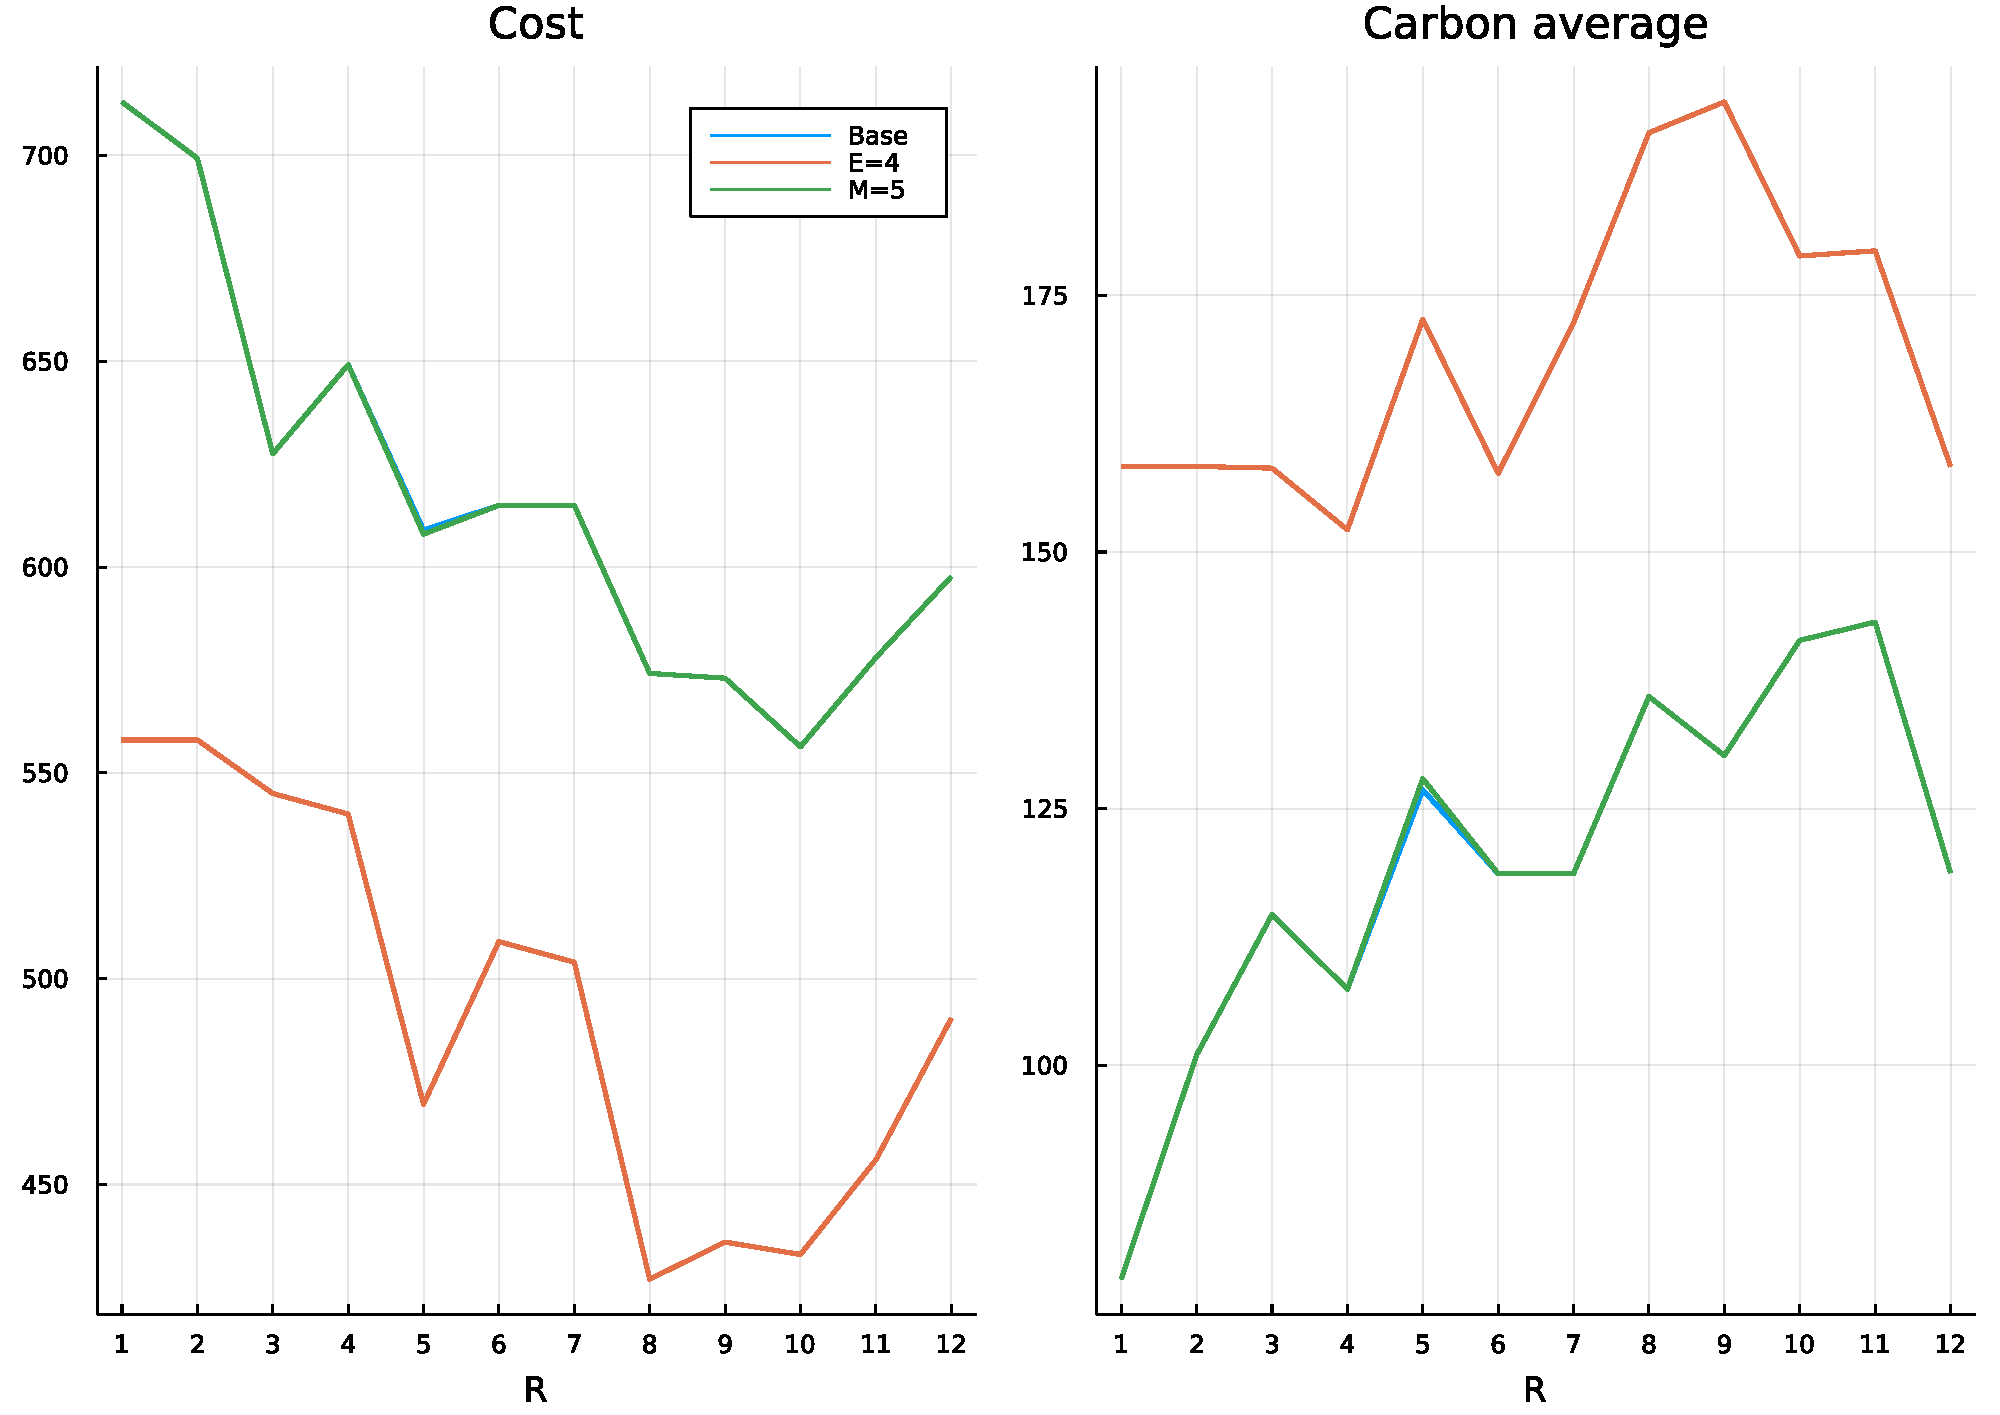
\includegraphics[width=\textwidth]{graph3.pdf}\\
	Ici on a ajouté le mode $f=50$ et $e=5$, on constate que les courbes verte et bleue sont quasi-superposées. Ce mode n'est presque pas utilisé, et donc les solutions sont inchangées.\\\newpage
	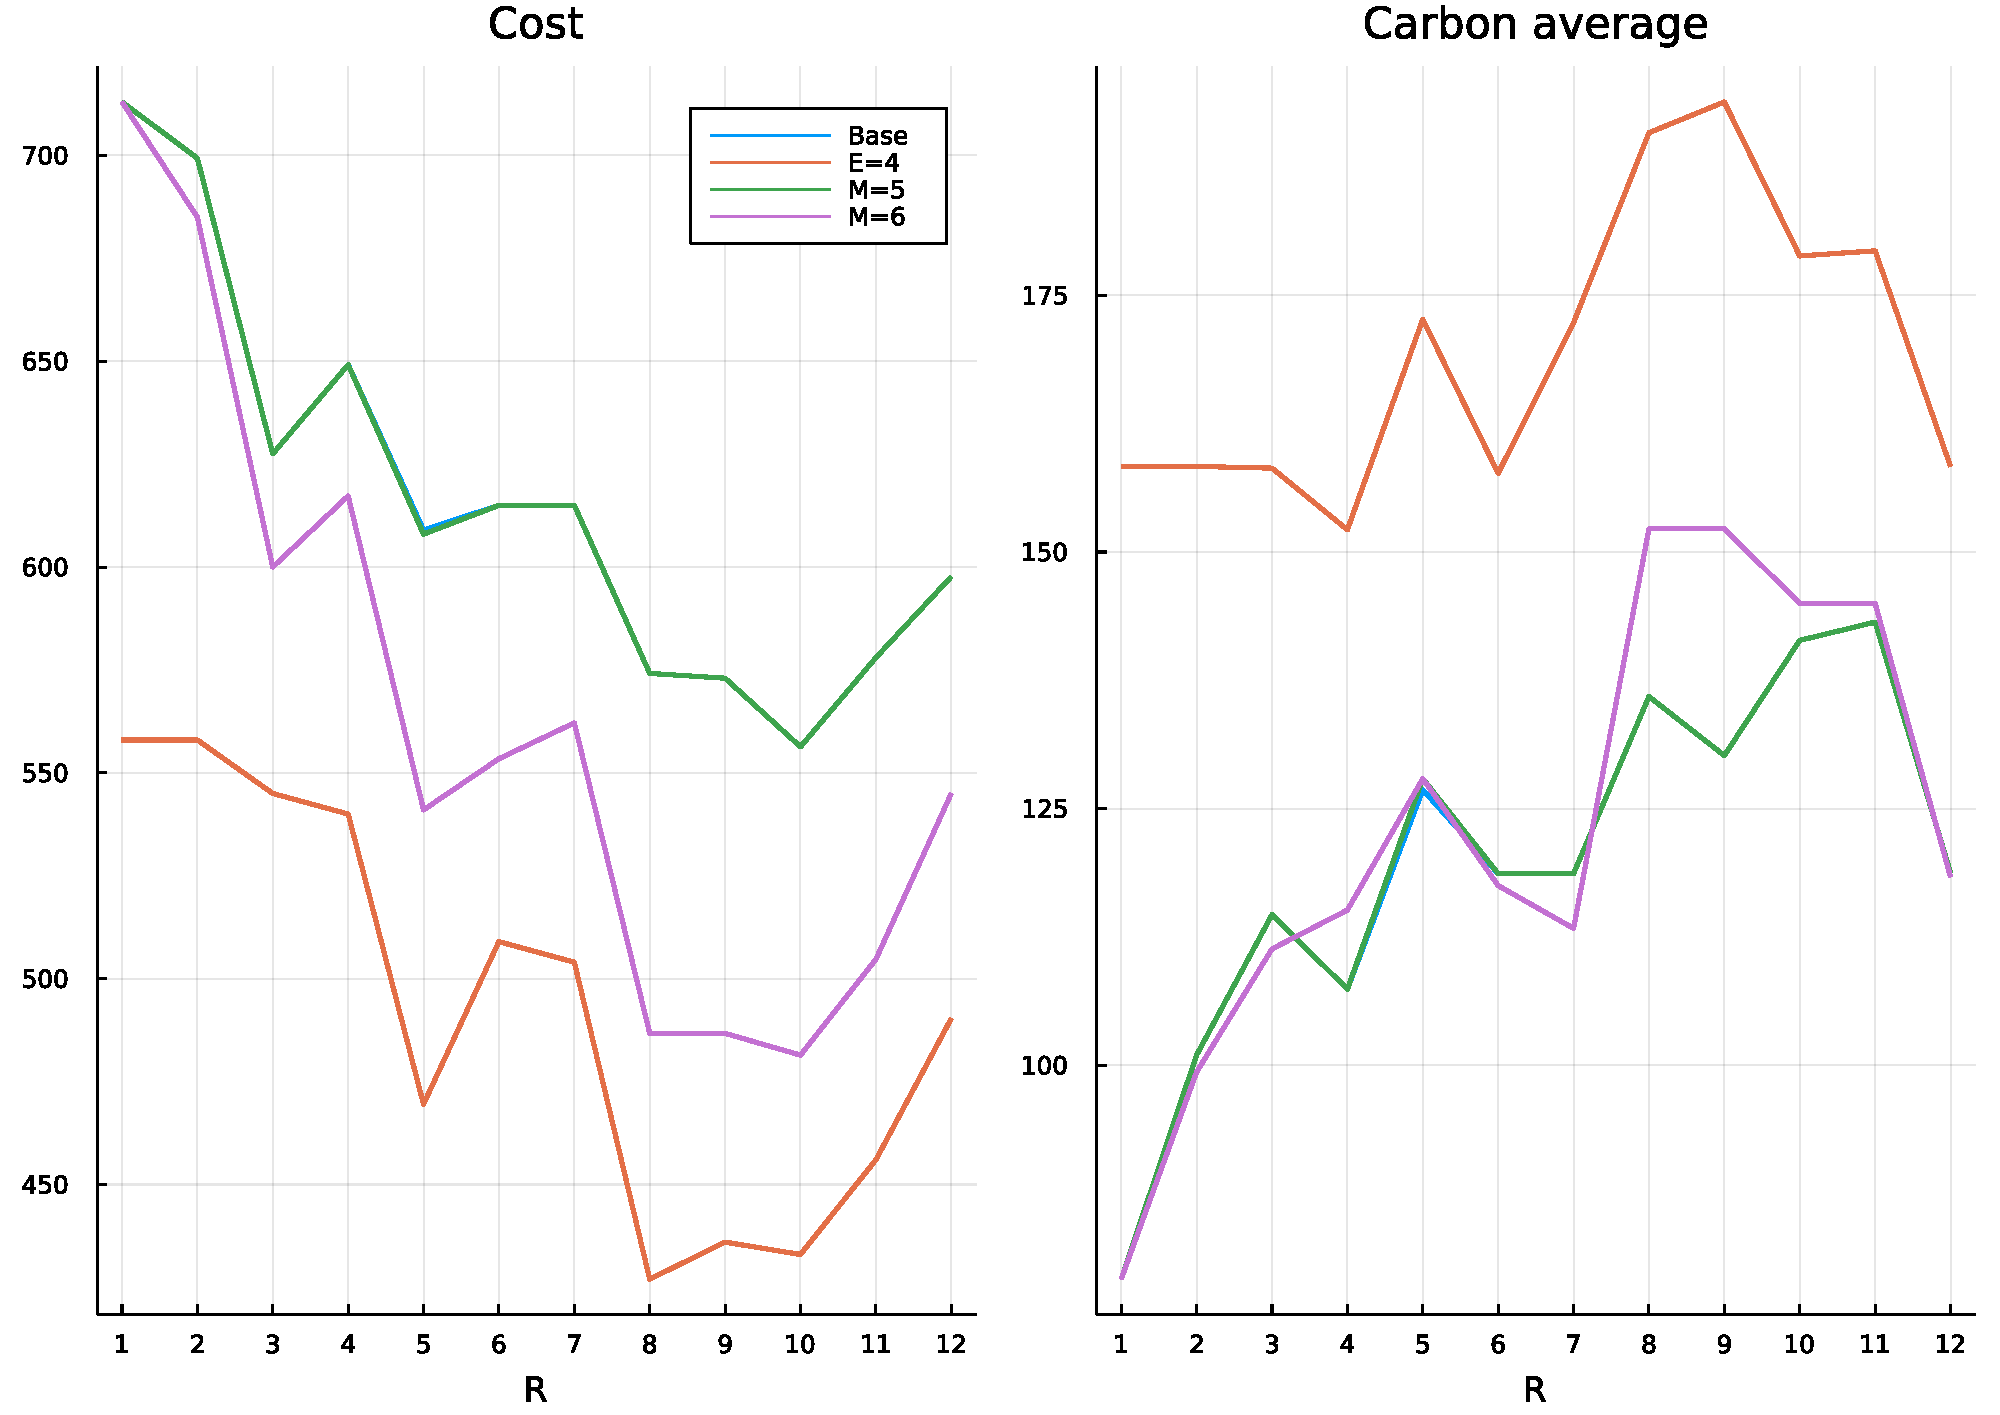
\includegraphics[width=\textwidth]{graph4.pdf}\\Ici on a ajouté le mode $f=95$ et $e=1$, on constate que la courbe violette est de coût toujours inférieur, puisqu'on ne peut avoir que de meilleures solutions étant donné que les solutions précédentes sont encore admissibles. On note que les émissions carbone n'ont pas particulièrement augmenté ou baissé.\\\newpage
	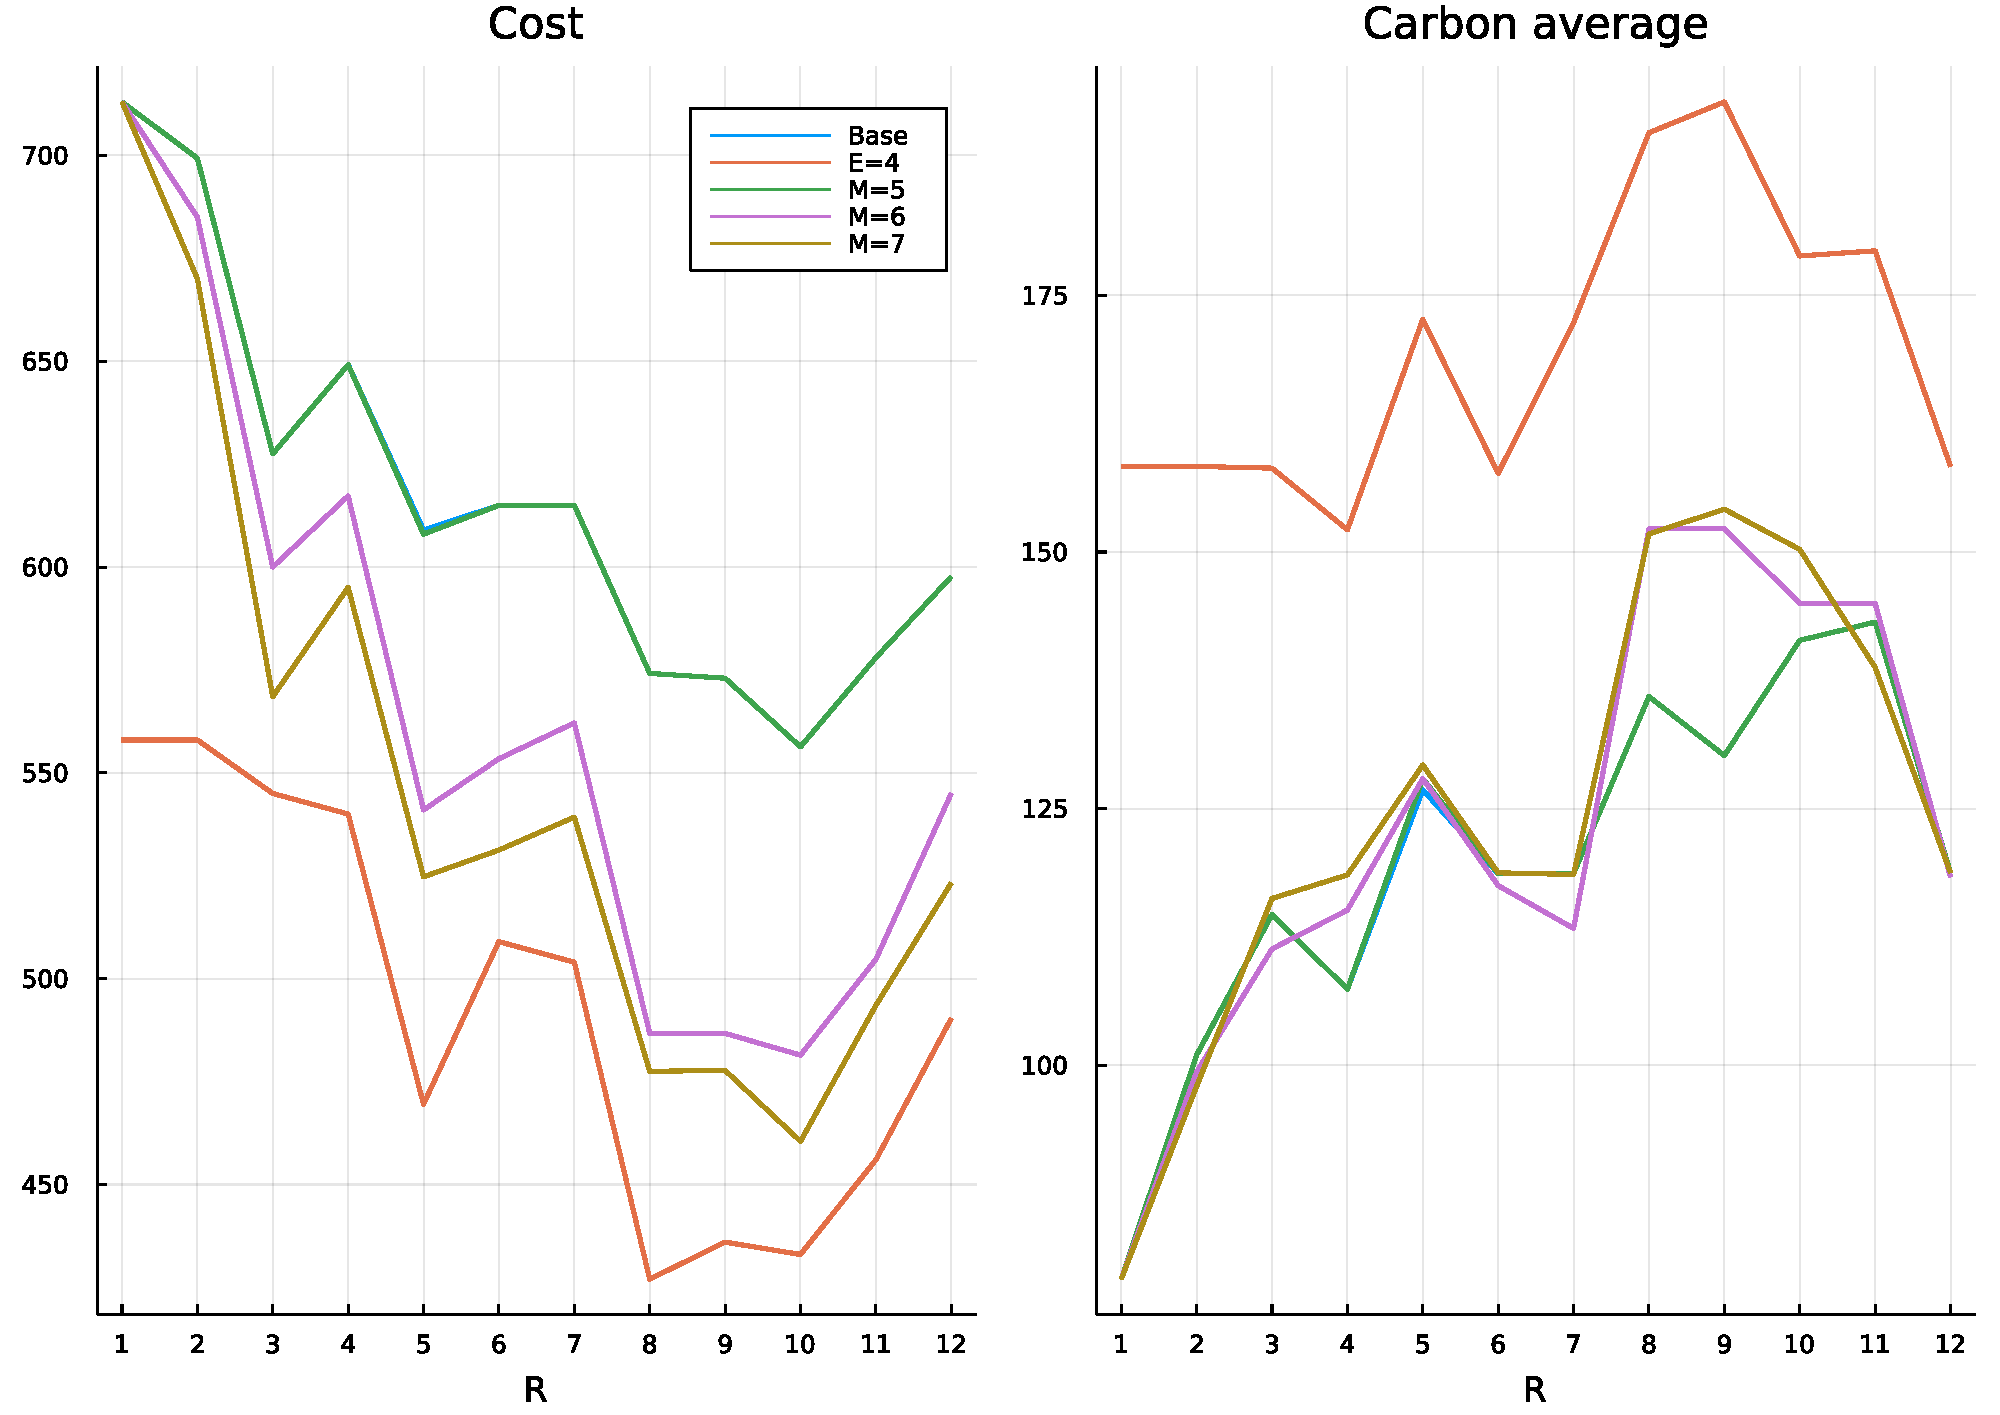
\includegraphics[width=\textwidth]{graph5.pdf}\\Ici on a ajouté le mode $f=1$ et $e=9$, et de la même manière, les coûts baissent et les émissions carbone sont similaires.\\
	Si on essaie d'estimer ce que devrait être l'émission de carbone moyenne, on peut déjà remarquer que à minima, la solution utilise le meilleur mode écologique. Dans ce cas, les émissions carbone sont d'en moyenne $\displaystyle{\sum_{t=1}^T d_t \frac{e}{T}}$ où $e$ est l'émission du meilleur mode écologique, au sens qu'il a un coût minimal. Cette valeur est d'environ 80 pour cette instance, ce qui est vérifié: lorsque $R=1$, on ne peut qu'utiliser un mode écologique et on a bien que la valeur de carbone pour $R=1$ est d'environ 80.\\
	Si on s'intéresse à la valeur moyenne, en faisant l'hypothèse que les émissions sont réparties uniformément sur le temps, alors on aurait $e=E$, et donc une valeur moyenne de $\displaystyle{\sum_{t=1}^T d_t \frac{E}{T}}$ ce qui donne environ 120, ce qui n'est pas aberrent au vu des résultats, qui avoisinent souvent cette valeur.\\
	\newpage
	Enfin, intéressons nous à l'influence de T. On pourrait s'attendre à ce que la valeur de T n'ait pas vraiment d'influence sur les deux valeurs, et en effet:\\
	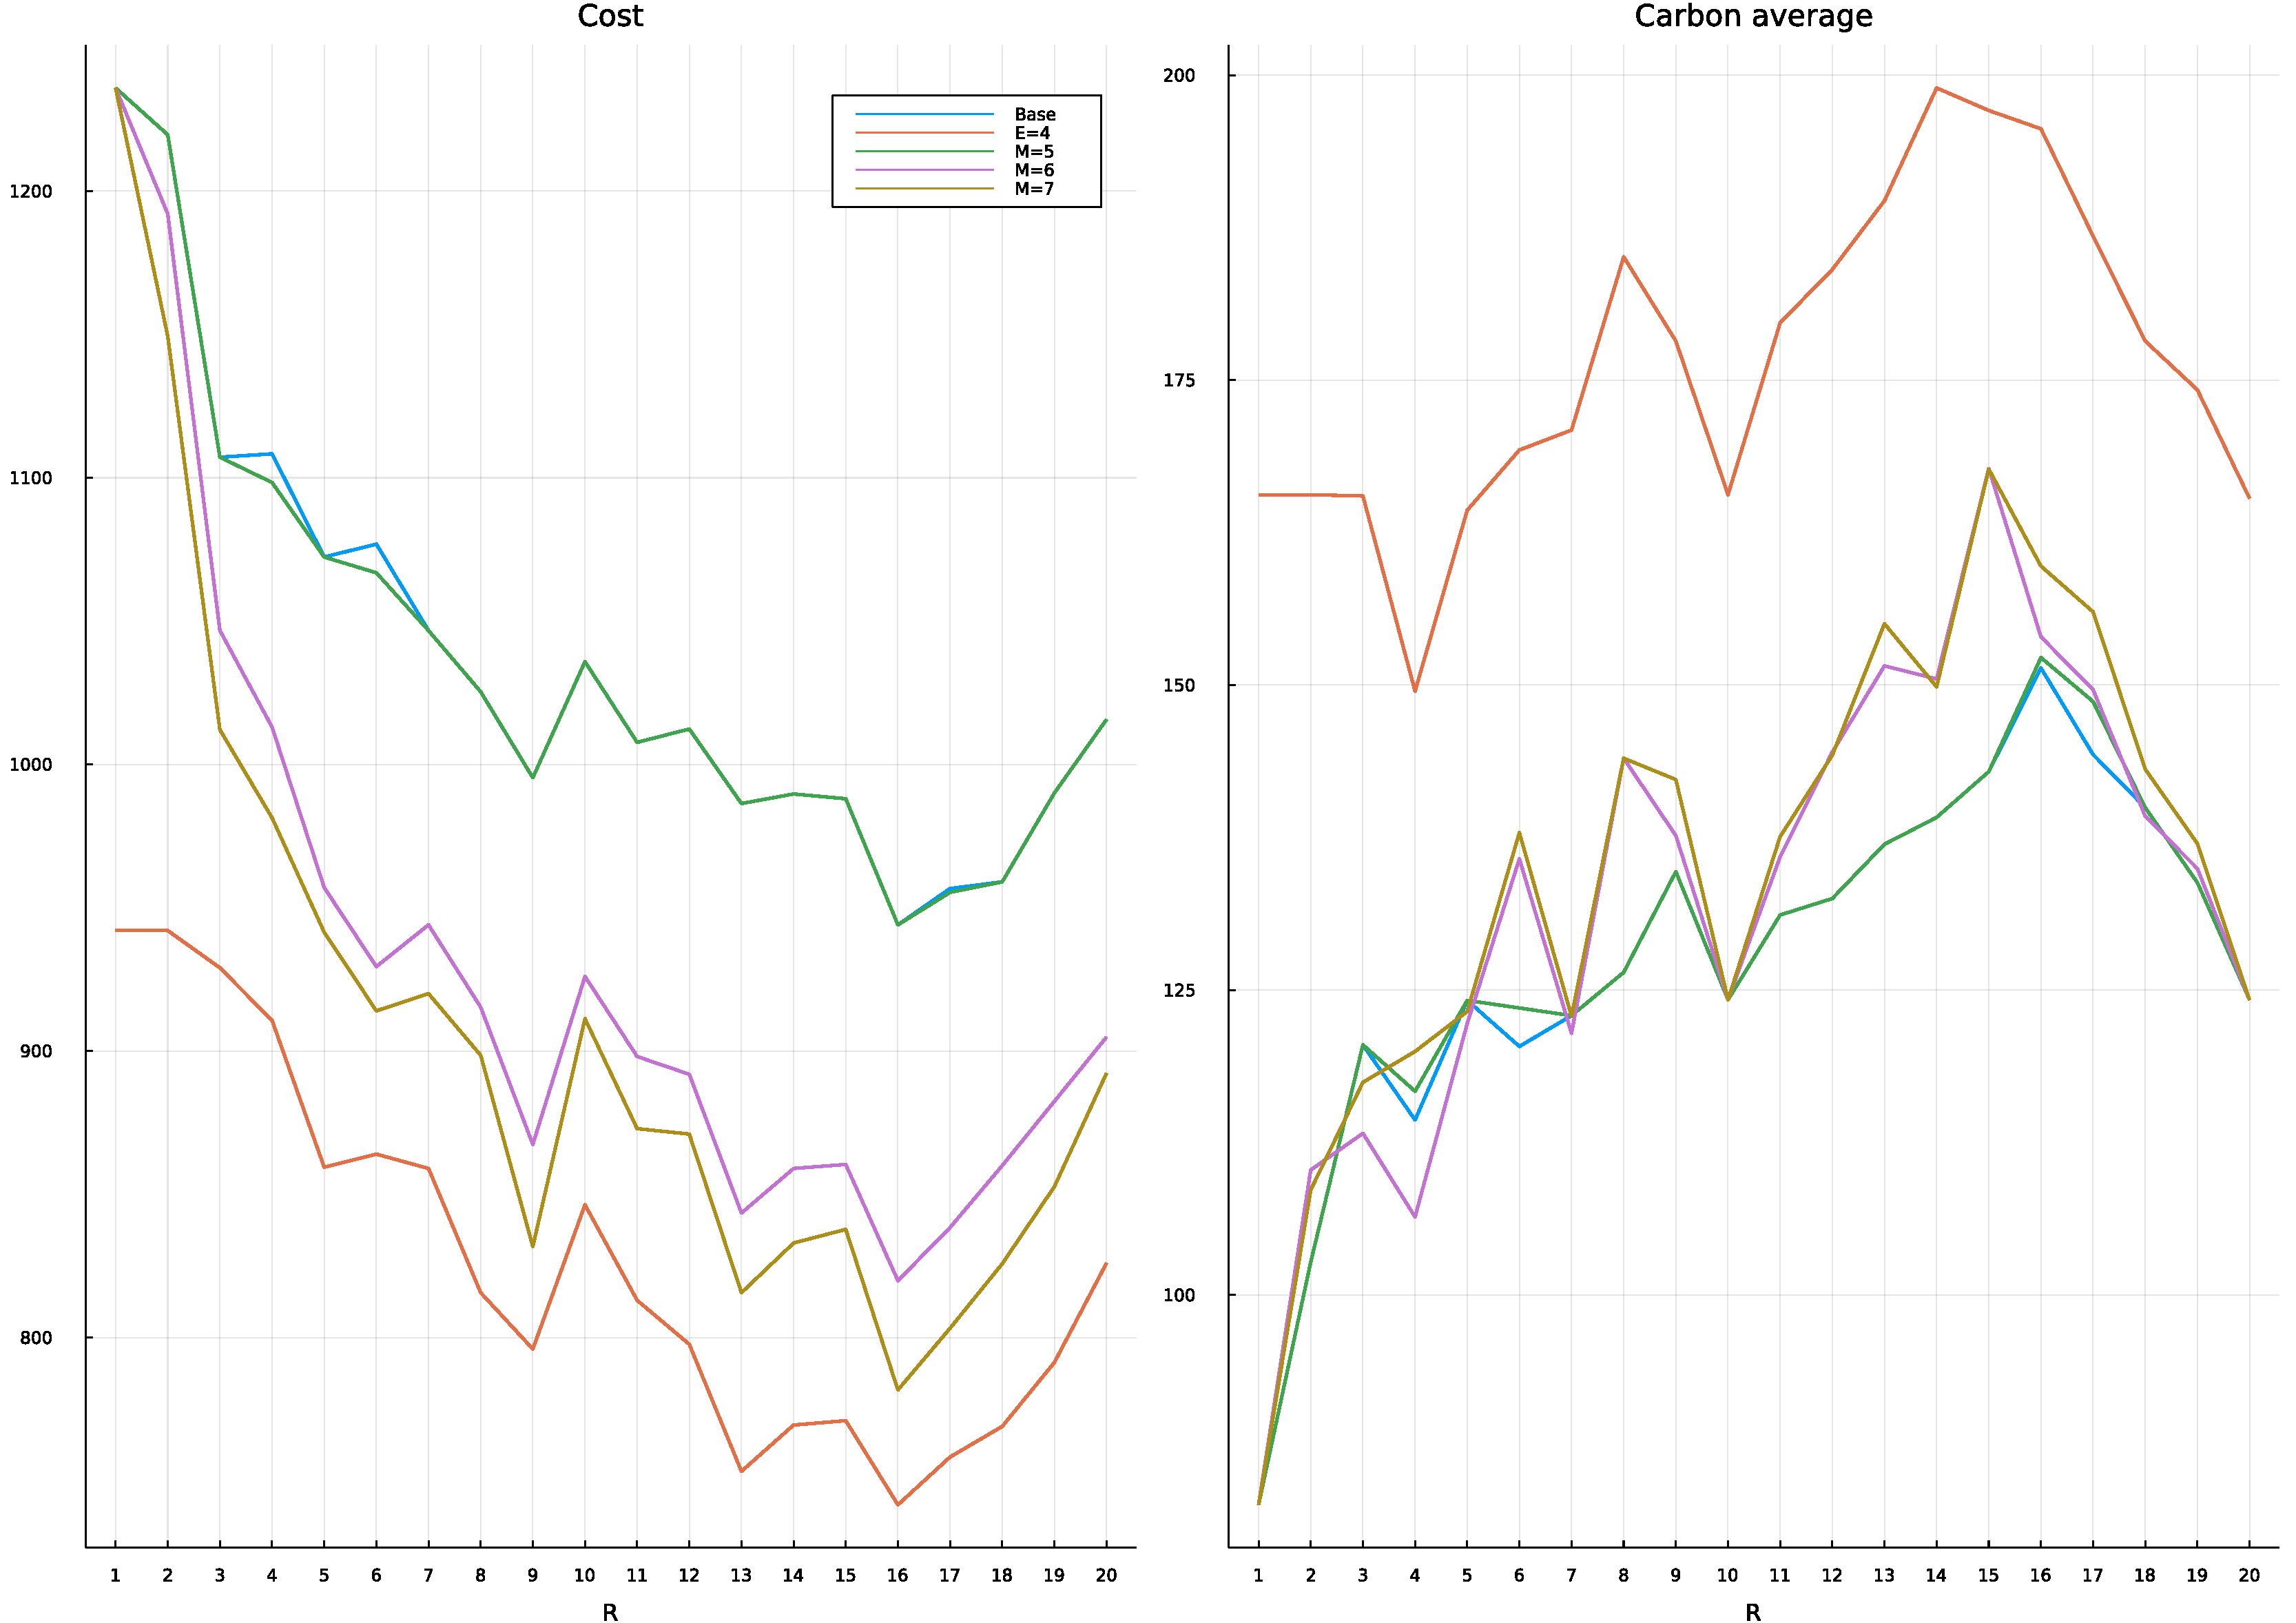
\includegraphics[width=\textwidth]{graph6.pdf}
	
	\section{Conclusion}
	En conclusion, on a adapté le modèle de dimensionnement de lot non contraint (ULS) en changeant la contrainte d'émission cumulée de carbone pour une contrainte glissante sur R périodes. On a constaté que lorsque R = 1 (contrainte périodique), les coûts sont élevés et les émissions carbone sont faibles. Tandis que lorsque R = T (contrainte globale), on remarque le contraire. Ce phénomène est d'ailleurs observé plus largement : lorsque R augmente, les coûts diminuent et les émissions carbones augmentent. Ce qui correspond bien au fait que lorsque R est grand, le problème est moins contraint. 
	On a également observé l'influence importante de $E_max$: lorsqu'il est grand, alors l'émission carbone est moins contrainte et donc augmente au profit des coûts. 
	Enfin, le type de mode disponible influence le comportement des solutions. Cependant, le plus souvent, la majorité des modes disponibles n'a pas d'impact sur la solution. La plupart du temps, seuls deux d'entre eux sont utilisés : un mode écologique et un mode économique.
	

\end{document}
